\subsection{Agente}
La implementación del componente Agente está escrito en rutinas de Sahi (ver sección \ref{sec-sahi}), primero se exponen los puntos relevantes en la implementación de las rutinas de respuesta y envío de órdenes de reposición para después señalar como se realizar la ejecución mediante la herramienta gráfica de Sahi.

\subsubsection{Rutina para automatizar la respuesta de órdenes de reposición}\label{sec-aut-contestar}
La rutina para automatizar la respuesta de órdenes de reposición refleja el caso de uso  CU-CONTESTAR que se describe en la sección \ref{cu-contestar}. A continuación se muestran las secciones de código más relevantes de la rutina que realizan la ejecución del caso de uso citado así como los subsecuentes (ver diagrama en la Figura \ref{fig:dia-casos-uso}). Los puntos relevantes en la implementación de la rutina son los siguientes:
\begin{enumerate}
	\item Ingresar al Sistema de Abastecimiento, en el Código \ref{lst:sah-session} se muestra la rutina para iniciar sesión en el Sistema de Abastecimiento:
	\begin{enumerate}
		\item Las líneas 1 y 2 se llenan los campos de usuario y contraseña.
		\item La línea 3 se envía el formulario.
		\item La línea 4 redirige a la pantalla con el listado de órdenes de reposición.  
	\end{enumerate}
	\begin{lstlisting}[language=Javascript, caption={Inicio de sesión en el Sistema de Abastecimiento.}, captionpos=b, label={lst:sah-session}]
_setValue(_textbox("Usuario[1]"), $user);
_setValue(_password("Contras[1]"), $pwd);
_click(_submit("Ingresar al Sistema"));
_click(_image("Normal[2]"));
	\end{lstlisting}

	\item Recolectar las órdenes de reposición listadas, el Código \ref{lst:sah-save-news} muestra un resumen de la automatización para guardar el listado de ordenes de reposición (ver caso de uso en la sección \ref{cu-guardar-nueva}):
	\begin{enumerate}
		\item La línea 1 muestra la declaración del ciclo para recorrer el listado de órdenes de reposición.
		\item Las líneas 2 a 4 muestran como se extrae el valor de los datos de una orden de reposición.
		\item Las líneas 5 a 7 muestran la obtención de las URLs para contestar y enviar las órdenes de reposición.
		\item La línea 8 es el almacenamiento de la nueva orden de reposición. 
	\end{enumerate}
	\begin{lstlisting}[language=Javascript, caption={Guardar lista de órdenes de reposición.}, captionpos=b, label={lst:sah-save-news}]
for(var $i = 1 + $errores; $i <= $rowCount; $i++){
	var $contrato = _getText(_table(1).rows[$i].cells[0]);
	var $solicitud = _getText(_table(1).rows[$i].cells[1]);
	var $numorden = _getText(_table(1).rows[$i].cells[2]);
	var $urlcon = "";
	_set($urlcon, _table(1).rows[$i].cells[6].childNodes[0].href);
	var $urlenv = $urlcon.replace("respoOra", "enviaOra");
	var $inserted = $persistence.insertOrden($contrato, $solicitud, $numorden, $expedicion, $almacen, $urlcon, $urlenv, $idSesion);
}
	\end{lstlisting}

	\item Contestar una a una cada orden de reposición, el Código \ref{lst:sah-respond} muestra un resumen de la automatización para contestar una orden de reposición (ver caso de uso en la sección \ref{cu-responder-orden}):
	\begin{enumerate}
		\item Las líneas 1 y 2 muestran como se redirige al explorador a la URL para contestar la orden de reposición.
		\item  Las líneas 3 muestran como se estable un valor en el formulario para contestar la orden de reposición.
		\item La línea 4 realiza el envío del formulario.
		\item La línea 5 manda la actualización de la orden de reposición en la base de datos.
	\end{enumerate}
	\begin{lstlisting}[language=Javascript, caption={Responder orden de reposición.}, captionpos=b, label={lst:sah-respond}]
var $url = $entidad.getUrlCon();
_navigateTo($url);
_setValue(_textbox("Lote"), "SL");
_click(_submit("Agregar Captura"));
$logica.updateCantidad($contrato, $numorden, $cantidad, $idSesion);
	\end{lstlisting}

	\item Enviar las órdenes de reposición contestadas, el Código \ref{lst:sah-send} muestra un resumen de la automatización para envíar una órden de reposición (ver caso de uso en la sección \ref{cu-enviar-orden}):
	\begin{enumerate}
		\item Las líneas 1 y 2 muestran como se redirige al explorador a la URL para enviar la orden de reposición.
		\item La líneas 3 a 6 crea un mapa con los datos de la orden de reposición.
		\item La línea 7 actualiza la orden de reposición en la base de datos. 
	\end{enumerate}
	\begin{lstlisting}[language=Javascript, caption={Enviar orden de reposición.}, captionpos=b, label={lst:sah-send}]
var $url = $entidad.getUrlEnv();
_navigateTo($url);
$mapa = new java.util.LinkedHashMap();
for(var $llave in $orden){
	$mapa.put($llave, $orden[$llave]);
}
$logica.updateOrden($mapa, $idSesion);
	\end{lstlisting}
\end{enumerate}

\subsubsection{Rutina para automatizar la verificación de órdenes de reposición canceladas}
La rutina para automatizar la verificación de órdenes de reposición canceladas refleja el caso de uso  CU-VERIFICAR que se describe en la sección \ref{cu-verificar}, a continuación se muestran las secciones de código más relevantes de la rutina que realizan la ejecución del caso de uso citado así como los subsecuentes (ver diagrama en la Figura \ref{fig:dia-casos-uso}). Los puntos relevantes en la implementación de la rutina son los siguientes:
\begin{enumerate}
	\item Ingresar al Sistema de Abastecimiento, el ingreso al sistema es idéntico a la rutina mostrada en la sección anterior (sección \ref{sec-aut-contestar}).

	\item Establecer los criterios de búsqueda, el Código \ref{lst:sah-search} muestra un resumen de la automatización para:
	\begin{enumerate}
		\item La línea 1 muestra la consulta de las fechas que acotan la búsqueda.
		\item Las líneas 2 a 5 realizan la búsqueda en el Sistema de Abastecimiento.
		\item Las líneas 6 y 7 extraen la información de las órdenes de reposición que muestra el Sistema de Abastecimiento como resultado de la búsqueda.
		\item Las líneas 8 y 9 utilizan el componente \textbf{Lógica de automatización} para actualizar en la base de datos el estado de las órdenes de reposición canceladas.
	\end{enumerate}
	\begin{lstlisting}[language=Javascript, caption={Responder orden de reposición.}, captionpos=b, label={lst:sah-search}]
$dateLimits = $logica.getDateLimits('dd/MM/yyyy');
_setSelected(_select("OrdStt"), "Canceladas");
_setValue(_textbox("OrdFeD"), $dateLimits[0]);
_setValue(_textbox("OrdFeA"), $dateLimits[1]);
_click(_submit(0));
var $html = '';
_set($html, _table(5).innerHTML);
$estado = $logica.getCancelStatus();
$logica.setSaiStatus($html, $estado, $idSesion);
	\end{lstlisting}
\end{enumerate}

\subsubsection{Ejecución de las rutinas de automatización}
La ejecución de las rutinas de sahi corresponden a los casos de uso CU-CONTESTAAR y 
CU-VERIFICAR (ver secciones \ref{cu-contestar} y \ref{cu-verificar} respectivamente), en ambos casos la ejecución es  
dejando la ejecución al usuario por medio de la interfaz gráfica de Sahi:
\begin{itemize}
	\item Iniciar Sahi sobre el explorar de Internet (ver Figura \ref{fig:ss-sahi-dashboard})
	\begin{figure}[h]
	\centering
	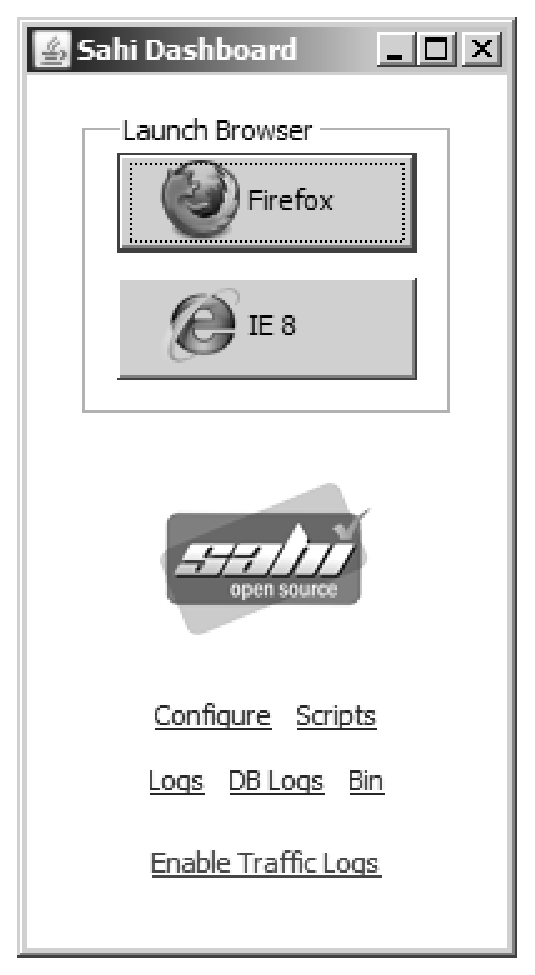
\includegraphics[scale=0.6]{ss-sahi-dashboard}
	\caption{Dashboard de Sahi.}
	\label{fig:ss-sahi-dashboard}
	\end{figure}

	\item Iniciar el controlador de Sahi y hacer los siguientes pasos (ver Figura \ref{fig:ss-sahi-controller}):
	\begin{enumerate}
		\item Seleccionar la rutina automatizada (contestar órdenes de reposición o verificación de órdenes de reposición)
		\item Ingresar la URL del Sistema de Abastecimiento
		\item Iniciar la ejecución.
	\end{enumerate}
	\begin{figure}[h]
	\centering
	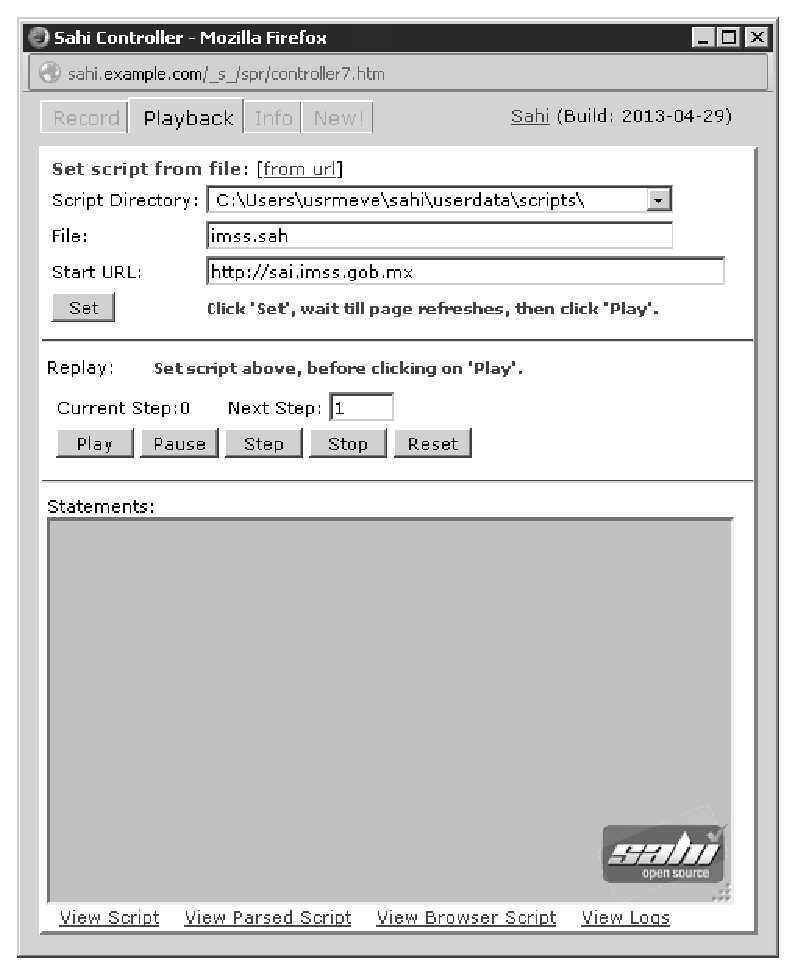
\includegraphics[scale=0.6]{ss-sahi-controller}
	\caption{Controlador de Sahi.}
	\label{fig:ss-sahi-controller}
	\end{figure}
\end{itemize}
